\section{Auswertung}
\label{sec:Auswertung}

\subsection{Wheatstonesche Brücke}
  Nachdem die die Widerstände jeweils so eingestellt wurden, dass die Brückenspannung 
  ihr Minimum erreicht, werden die in Tabelle \ref{tab:some} dargestellten Werte für 
  die Widerstände aufgenommen. Anhand dieser kann nach Gleichung ... der zu untersuchende
  Widerstände $R_x$ bestimmt werden.
  \begin{table}[H]
    \centering
    \caption{Messwerte der Wheatstoneschen Brücke}
    \label{tab:some}
    \begin{tabular}{c c c c}
     \toprule
      $R_2 $[\si{\ohm}] & $R_3$ [\si{\ohm}] & $R_4 $[\si{\ohm}]& $R_x $[\si{\ohm}]\\
     \midrule
     500 & 390 & 610 & 319.672 \\
     332 & 490 & 510 & 318.98  \\
     1000 & 242 & 758 & 319.261 \\
     \bottomrule
    \end{tabular}
  \end{table} 
  Der Mittelwert dieser für $R_x$ bestimmten Werte wurde mit numpy ermittelt und lautet
  $R_x= 319.3 \pm 0.28$. 

\subsection{Kapazitätsmessbrücke}
  Bei der Kapazitätsmessbrücke wird für ein Bauteil mit unbekanntem Widerstand $R_x$
  und unbekannter Kapazität $C_x$ das Minimum des Brückenstroms durch eine Konstellation 
  mit den folgenden Werten erreicht.
  \begin{align*}
    R_2 = \SI{228.5}{\ohm}\\
    R_3 = \SI{632}{\ohm}\\
    R_4 = \SI{386}{\ohm}\\
    C_2 = \SI{750}{\nano\farad}\\
  \end{align*}
  Daraus kann durch Gleichung ... auf
  \begin{align*}
    R_x = \SI{391.5}{\ohm}\\
    C_x = \SI{436.7}{\nano\farad}\\
  \end{align*}
  geschlossen werden.

\subsection{Induktivitätsbrücke}
  Bei dieser Brückenschaltung werden zu dem Bauteil $R_x$ $L_x$ die folgenden Wiederstände 
  und Induktivität festgestellt:
  \begin{align*}
    R_2 = \SI{224}{\ohm}\\
    R_3 = \SI{608}{\ohm}\\
    R_4 = \SI{392}{\ohm}\\
    L_2 = \SI{20.1}{\milli\henry}
  \end{align*}
  Aus diesen ergeben sich für $R_x = 375.34 \si{\ohm}$ und $L_x = 31.17 \si{\milli\henry}$.
  
\subsection{Maxwell-Brücke}
  Das selbe Bauteil wird nun in einer Maxwell-Brückenschaltung untersucht. Hier ergeben 
  sich die folgenden Werte:
  \begin{align*}
    R_2=332\si{\ohm}\\
    R_3 = 191 \si{\ohm}\\
    R_4 = 179 \si{\ohm}\\
    C_2 = 750 \si{\milli\farad}
    R_x = 354.25 \si{\ohm}\\
    L_x = 47.5 \si{\milli\henry}
  \end{align*}

\subsection{Wien-Robinson-Brücke}
  Bei einem Widerstand von $R=1000 \si{\kilo\ohm}$, einer Kapazität von $C = 295 \si{\nano\farad}$
  werden folgende Werte gemessen:
  \begin{table}[H]
    \centering
    \caption{Messdaten zur Wien-Robinson-Brücke}
    \label{tab:some}
    \begin{tabular}{c c}
     \toprule
      $\nu$ [Hz] & Amplitude [V]\\
     \midrule
     20 & 3.2    \\
     120 & 2.75   \\
     220 & 1.875  \\
     320 & 1.125  \\
     420 & 0.52   \\
     500 & 0.17   \\
     520 & 0.0775 \\
     530 & 0.04   \\
     540 & 0.005  \\
     550 & 0.04   \\
     600 & 0.225  \\
     700 & 0.56   \\
     800 & 0.75   \\
    1000 & 1.25   \\
    2000 & 2.5    \\
    3000 & 2.7    \\
    4000 & 2.85   \\
    5000 & 2.95   \\
    10000 & 3      \\
    15000 & 2.7    \\
    20000 & 2.3    \\
    \bottomrule
    \end{tabular}
  \end{table} 
  Diese sind in Abbildung \ref{fig:plot} grafisch dargestellt.
  \begin{figure}
      \centering
      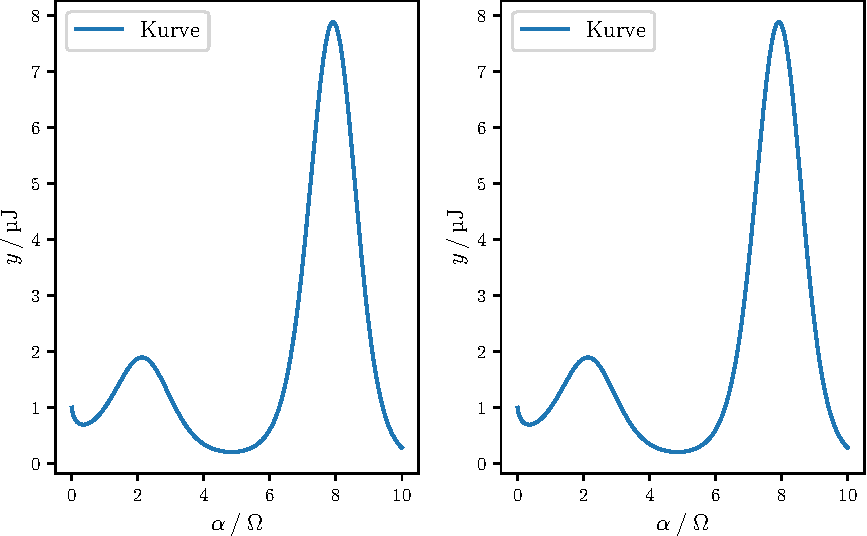
\includegraphics{plot.pdf}
      \caption{Messdaten zur Wien-Robinson-Brücke}
    \label{fig:plot}
  \end{figure}


